\section{启动空白操作系统}

\subsection{操作系统启动流程}

按下电源键后计算机开始启动,启动过程分为3个阶段~\cite{阮一峰2014如何变得有思想}:
\begin{center}BIOS -> MBR -> 操作系统\end{center}

\begin{enumerate}
\item 在BIOS完成POST(硬件自检,Power-On Self Test)
  并根据启动顺序(Boot Sequence)来选择启动设备。本系统是从U盘启动。
\item 计算机读取该设备的MBR(Master boot record,位于第一个扇区,即最前面的512个字节,见图~\ref{fig:mbr}),
  并运行其中的启动程序IPL(Initial Program Loader),将ZOS加载入内存。
  本部分的实现代码,参见附录程序~\ref{sec:ipl09}。
\item 控制权转交给操作系统后,Kernel开始运行,操作系统启动完成。
\end{enumerate}

\subsection{制作MBR}

MBR的主要部分是Bootstrap code area,即前446个字节。MBR结构见图~\ref{fig:mbr}。
负责指出操作系统的位置,主分区第一个扇区的物理位置(柱面、磁头、扇区号等等)
,参见附录程序\ref{sec:fat12}。

\begin{figure}[H]
  \centering
  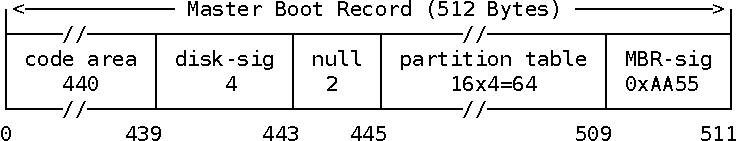
\includegraphics[width=1\textwidth]{fig/mbr.pdf}
  \caption{MBR}
  \label{fig:mbr}
\end{figure}

一个扇区大小为512字节,MBR位于C0-H0-S1(柱面0,磁头0,扇区1),\cite{刘伟2010数据恢复技术深度揭秘}
从下一个扇区(扇区2,C0-H0-S2)开始加载操作系统。找到扇区2的操作如程序~\ref{lst:chs}所示。

\begin{listing}[H]
  \begin{codeblock}[.5]
  \inputminted[tabsize=2, firstline=43, lastline=45,
  linenos=true]{nasm}{../ZOS/src/kernel/ipl09.nas}
  \end{codeblock}
  \caption{初始化读取柱面、磁头和扇区的起点}
  \label{lst:chs}
\end{listing}

完成定位后开始将磁盘数据读入内存,策略是
\begin{enumerate}
\item 磁头0,柱面0,读取1-18扇区 (C0-H0-S2)-(C0,H0,S18)
\item 磁头1,柱面0,读取1-18扇区 (C0-H1-S1)-(C0-H1-S18)
\item 磁头0,柱面1,读取1-18扇区 (C1-H0-S1)-(C1-H0-S18)
\item ...
\item 磁头1,柱面78,读取1-18扇区 (C78-H1-S1)-(C78-H1-S18)
\item 磁头0,柱面79,读取1-18扇区 (C79-H0-S1)-(C79-H0-S18)
\item 磁头1,柱面79,读取1-18扇区 (C79-H1-S1)-(C79-H1-S18)
\end{enumerate}

按以上策略将磁盘内容读入内存,核心代码如附录程序~\ref{sec:readfrag}。

readfast 位于代码第76行,JMP readfast 在此代表循环执行。
当循环执行完毕,表示磁盘内容已经全部加载到内存中,
MBR过程成功,开始启动操作系统。

\subsection{制作空白操作系统}

为测试操作系统是否成功被MBR启动,设计将操作系统设置为启动后待机。
如程序~\ref{lst:blankos}所示。按下电源键,经过启动步骤系统循环执行
HLT\footnote{HLT: 让CPU停止动作并进入待机状态\cite{30_osKawaiHidemi200630}}
使得操作系统计算机始终处于待机状态,启动成功。

\begin{listing}[H]
  \begin{codeblock}[.5]
    \begin{nasmcode}
      fin:
      HLT
      JMP fin
    \end{nasmcode}
  \end{codeblock}
  \caption{空白操作系统}
  \label{lst:blankos}
\end{listing}

\section{操作系统组件功能全览}
在完成空白操作系统后,操作系统的设计才正式拉开序幕,
此次为操作系统设计的功能如图~\ref{fig:run}所示,
操作系统启动后将完成各种功能需求的初始化操作,
在初始化成功后各项功能就可以正常运行。

\begin{figure}[H]
  \centering
  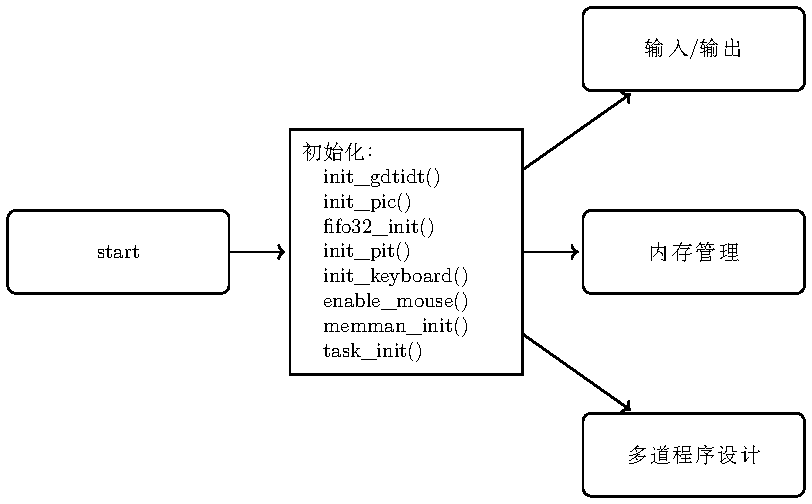
\includegraphics[width=.8\textwidth]{fig/func/run.pdf}
  \caption{操作系统组件功能全览}
  \label{fig:run}
\end{figure}

\begin{description}
  \item[初始化] 初始化过程主要涉及到:\\
  内存的损坏检测,数据情况,系统数据写入;\\
  输入设备中键盘及鼠标的启用等;
  \item[内存管理] 内存管理包括内存的分配和释放;
  \item[输入输出] 输入输出包括键盘输入,鼠标输入,标准输出;
  \item[多道程序] 多道程序中设计多道程序设计,分时系统,程序切换及程序的优先级设置。
\end{description}